\documentclass[a4paper]{article}

\usepackage[T3]{fontenc}
\usepackage[utf8]{inputenc}
\usepackage[russian]{babel}

\usepackage{fullpage} % Package to use full page
\usepackage{parskip} % Package to tweak paragraph skipping

\usepackage{amsmath, amssymb}
\usepackage{graphicx}
\usepackage[colorinlistoftodos]{todonotes}

\usepackage{gensymb} % для значка градуса

\usepackage{mhchem}

\begin{document}

\begin{titlepage}
\centering
\textbf{\large Московский государственный университет имени М.В.\,Ломоносова\\
\vspace*{0.1cm} Химический факультет\\
\vspace*{0.1cm}
\noindent\makebox[\linewidth]{\rule{\paperwidth}{0.4pt}}
\vspace*{0.1cm}
 Кафедра органической химии\\
\vspace*{0.1cm} Лаборатория супрамолекулярной химии и нанотехнологии органических материалов \\}
\vspace*{2cm}

\begin{center}

\includegraphics[width=0.3\textwidth]{pictures/logo.jpg}
\end{center}

\vspace*{2cm}
\Large \textbf{Синтез (2E, 2$^\prime$E)-бензол-1,4-диил-ди(Е)-метилиден)дициклопентанона.}
\vspace*{2cm}

\begin{flushright}
\large Курсовая работа студента 311 группы\\
Финенко А.А.\\
\vspace{1cm}
Научный руководитель:\\
к.х.н., доц. Нуриев В.Н.
\end{flushright}
\vfill
\large\textbf{Москва\\ 2016}
\end{titlepage}

\tableofcontents

\begin{abstract}
Abstract.
\end{abstract}

\section{Синтез 2-бензолиденциклопентанона.}
\begin{center}
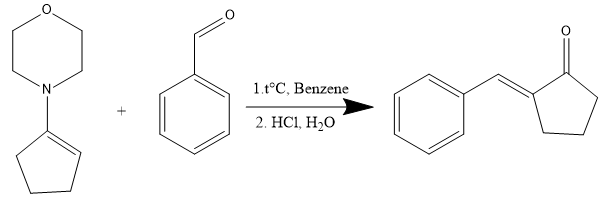
\includegraphics[scale=0.5]{pictures/1.png}
\end{center}
11.45г (74.84 ммоль) N-циклопентанилморфолина, 6.61г (62.36 ммоль) свежеперегнанного бензальдегида и 60 мл бензола помещают в круглодонную колбу и нагревают с насадкой Дина-Старка в течение 20 часов. За ходом реакции следят при помощи ТСХ (элюент -- петролейный эфир : этилацетат, 4 : 1).
Затем раствор охлаждают до комнатной температуры и при перемешивании добавляют 43.5 мл 6М $\ce{HCl}$. После перемешивания в течение 2 часов органический слой отделяют и промывают водой до нейтрального pH, оставляют сушиться над $\ce{Na2SO4}$ на ночь. Затем смесь фильтруют и отгоняют бензол на роторном растворителе. Остаток охлаждают и кристаллизуют. Очистку производят перекристаллизацией из смеси этанол - циклогексан.
%\addcontentsline{toc}{section}{}

<<<<<<< 855873ef033897de82c2dfa0b3e0ec7e15897d5e
\section*{Синтез 2-бензолиден-5-(4-метоксибензолиден)циклопентанона.}
=======
\section{Синтез 2-бензолиден-5-(4-метоксибензолиден)циклопентанона.}
>>>>>>> interim
\begin{center}
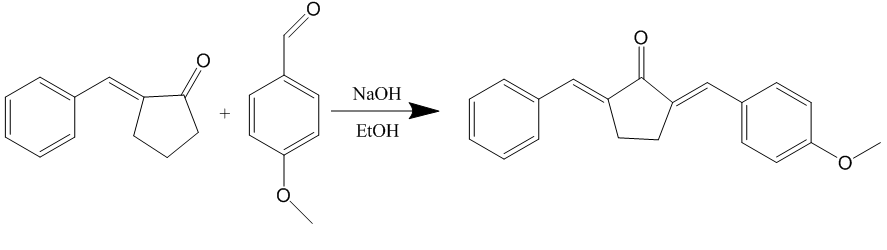
\includegraphics[scale=0.35]{pictures/2.png}
\end{center}
172 мг  моноенона, 136 мг анисового альдегида, 230 мкл 2N $\ce{NaOH}$ и 1.5мл $\ce{EtOH}$ помещают в круглодонную колбу и перемешивают в течение часа. Реакция протекает при комнатной температуре, за ходом реакции следят при помощи ТСХ. Реакция сопровождается выпадением грязно-желтого осадка диенона. После окончания реакции реакционную смесь переносят на фильтр со стеклянным фильтрующим дном, осадок промывают небольшими количествами воды, сушат в пистолете Фишера. 
Выход: 40.69$\%$ (от теории).

<<<<<<< 855873ef033897de82c2dfa0b3e0ec7e15897d5e
\section*{Синтез 2-бензолиден-5-(пиридин-3-илметилен)циклопентанона.}
=======
\section{Синтез 2-бензолиден-5-(пиридин-3-илметилен)циклопентанона.}
>>>>>>> interim
\begin{center}
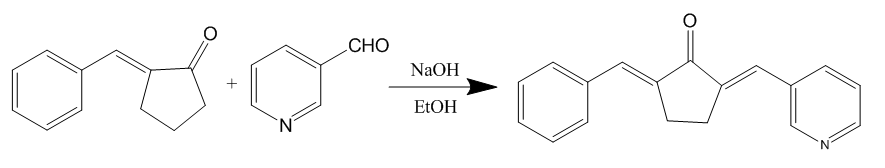
\includegraphics[scale=0.35]{pictures/3.png}
\end{center}
172 мг моноенона, 107 мг 3-пиридинкарбальдегида, 330 мкл 2N $\ce{NaOH}$ и 1.5 мл $\ce{EtOH}$ помещают в круглодонную колбу и перемешивают в течение часа. Реакция протекает при комнатной температуре, за ходом реакции следят при помощи ТСХ. Реакция сопровождается выпадением оранжево-желтого осадка диенона. После окончания реакции реакционную смесь переносят на фильтр со стеклянным фильтрующим дном, осадок промывают небольшими количествами воды, сушат в пистолете Фишера.
Выход: 44.83$\%$ (от теории).

\section{Синтез бензол-1,4-диил-диметилидендициклопентанона.}
К раствору 50 ммоль 1-морфолиноциклопентена в 50 мл бензола добавляют 2-3 капли морфолина и 50 мг п-толуолсульфокислоты. Смесь кипятят с насадкой Дина-Старка до прекращения выделения воды (30-60 минут). Затем к смеси добавляют 25 ммоль терефталевого альдегида, интенсивно перемешивают и кипятят с азеотропной отгонкой воды 12-14 часов, в результате чего получается черная смолообразная смесь. После охлаждения к смеси прибавляют 20 мл конц. $\ce{HCl}$ и перемешивают при 20$^{\circ}$ в течение 3 часов. Продукт экстрагируют $\ce{CH2Cl2}$, объединенные вытяжки сушат над $\ce{Na2SO4}$ и упаривают в роторном испарителе. Затем готовят смесь остатка с минимальным количеством силикагеля (до получения пересыпчатого порошка) и проводят флэш-хроматографию с элюентом $\ce{EtOAC}$ - $\ce{C6H14}$ (с плавным возрастанием полярности от 1:5 до 3:1). Получают 34.89$\%$ целевого диенона. \\ $T = 181-184^{\circ}$.
Спектр $^{1}$H-NMR ($\ce{CDCl3}$):  $\delta$ 2.04 (4H, m, 2 $\times$ $C4-H_{2}$), 2.40 (4H, t, \textit{J} = 7.9 Гц, 2 $\times$ $C5-H_{2}$), 2.96--3.00 (4H, m, 2 $\times$ $C3-H_{2}$), 7.35 (2H, t, \textit{J} = 2.57 Гц, винильные H), 7.56 (4H, s, арильные H).

\end{document}